\section{configobj::Config\-Obj\-Error Class Reference}
\label{classconfigobj_1_1ConfigObjError}\index{configobj::ConfigObjError@{configobj::ConfigObjError}}
Inheritance diagram for configobj::Config\-Obj\-Error::\begin{figure}[H]
\begin{center}
\leavevmode
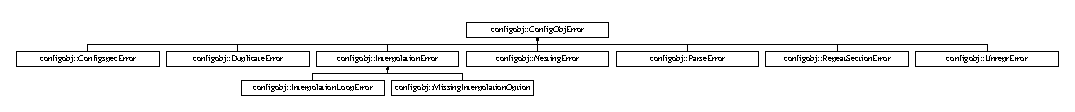
\includegraphics[height=1.05727cm]{classconfigobj_1_1ConfigObjError}
\end{center}
\end{figure}
\subsection*{Public Member Functions}
\begin{CompactItemize}
\item 
def \textbf{\_\-\_\-init\_\-\_\-}\label{classconfigobj_1_1ConfigObjError_f5287b5e65a96bff3310a78f79582807}

\end{CompactItemize}
\subsection*{Public Attributes}
\begin{CompactItemize}
\item 
\textbf{line}\label{classconfigobj_1_1ConfigObjError_8f4cc54a73c7b5381515a42531c270af}

\item 
\textbf{line\_\-number}\label{classconfigobj_1_1ConfigObjError_17f84e438edc4fb0805a9c6547569b63}

\item 
\textbf{message}\label{classconfigobj_1_1ConfigObjError_2ccd77b0d14701e8ead308b7a66de43e}

\end{CompactItemize}


\subsection{Detailed Description}


\footnotesize\begin{verbatim}
This is the base class for all errors that ConfigObj raises.
It is a subclass of SyntaxError.
\end{verbatim}
\normalsize
 



The documentation for this class was generated from the following file:\begin{CompactItemize}
\item 
old/PANICtool-1.0/configobj.py\end{CompactItemize}
